% Source: graduate-coursework/Research/How_to_write/00_Contrastive_Synthesis.tex
% Description: \textbf{Cognitive Process Theory (Flower \& Hayes, 1981).

\documentclass[border=4pt]{standalone}
\usepackage{newtxtext,newtxmath}
\usepackage{tikz}
\usetikzlibrary{arrows.meta,positioning,shapes.geometric,calc,decorations.pathreplacing}

\definecolor{garnet}{HTML}{73000A}
\definecolor{atlantic}{HTML}{466A9F}
\definecolor{congaree}{HTML}{1F414D}
\definecolor{horseshoe}{HTML}{65780B}
\definecolor{rose}{HTML}{CC2E40}
\definecolor{honeycomb}{HTML}{A49137}
\definecolor{warmgrey}{HTML}{676156}
\definecolor{black90}{HTML}{363636}
\definecolor{black70}{HTML}{5C5C5C}
\definecolor{black50}{HTML}{A2A2A2}
\definecolor{black30}{HTML}{C7C7C7}
\definecolor{black10}{HTML}{ECECEC}
\definecolor{sandstorm}{HTML}{FFF2E3}

\begin{document}
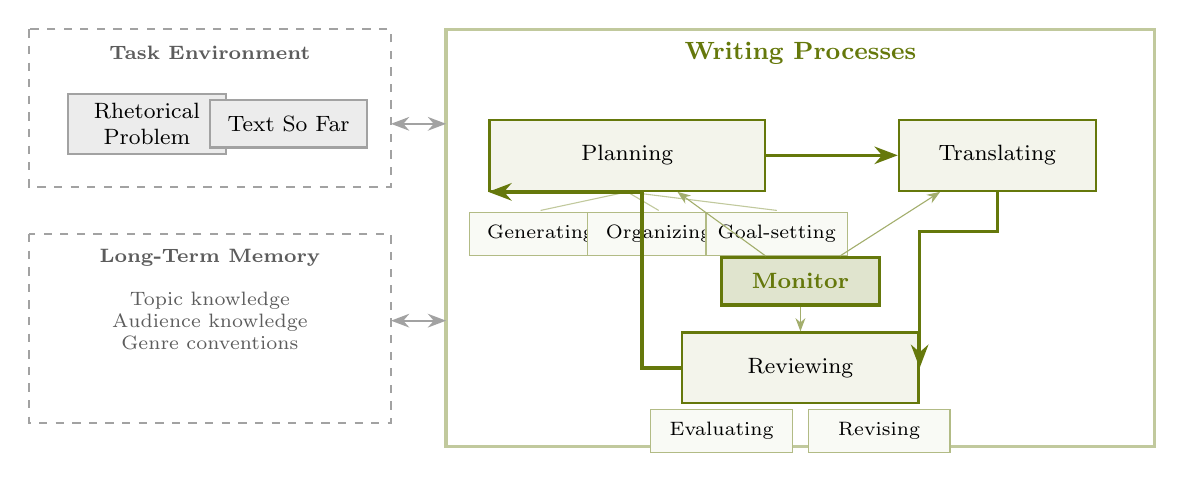
\begin{tikzpicture}[
    every node/.style={font=\footnotesize},
    box/.style={rectangle, draw=horseshoe, thick, fill=horseshoe!8,
        minimum width=2.5cm, minimum height=0.9cm, align=center, font=\footnotesize},
    subbox/.style={rectangle, draw=horseshoe!50, fill=horseshoe!4,
        minimum width=1.8cm, minimum height=0.55cm, align=center, font=\scriptsize},
    envbox/.style={rectangle, draw=black50, thick, fill=black10,
        minimum width=2.5cm, minimum height=0.9cm, align=center, font=\footnotesize},
]

% Task Environment
\draw[thick, black50, dashed] (-6.8, 3.8) rectangle (-2.2, 1.8);
\node[font=\scriptsize\bfseries, text=black70] at (-4.5, 3.5) {Task Environment};
\node[envbox, minimum width=2cm, minimum height=0.6cm] at (-5.3, 2.6) {Rhetorical\\Problem};
\node[envbox, minimum width=2cm, minimum height=0.6cm] at (-3.5, 2.6) {Text So Far};

% Long-Term Memory
\draw[thick, black50, dashed] (-6.8, 1.2) rectangle (-2.2, -1.2);
\node[font=\scriptsize\bfseries, text=black70] at (-4.5, 0.9) {Long-Term Memory};
\node[font=\scriptsize, text=black70, align=center] at (-4.5, 0.1) {Topic knowledge\\Audience knowledge\\Genre conventions};

% Writing Processes box
\draw[very thick, horseshoe!40] (-1.5, 3.8) rectangle (7.5, -1.5);
\node[font=\small\bfseries, text=horseshoe] at (3, 3.5) {Writing Processes};

% Planning
\node[box, minimum width=3.5cm] (plan) at (0.8, 2.2) {Planning};
\node[subbox] at (-0.3, 1.2) {Generating};
\node[subbox] at (1.2, 1.2) {Organizing};
\node[subbox] at (2.7, 1.2) {Goal-setting};
\draw[thin, horseshoe!40] (plan.south) -- (-0.3, 1.5);
\draw[thin, horseshoe!40] (plan.south) -- (1.2, 1.5);
\draw[thin, horseshoe!40] (plan.south) -- (2.7, 1.5);

% Translating
\node[box] (trans) at (5.5, 2.2) {Translating};

% Reviewing
\node[box, minimum width=3cm] (rev) at (3, -0.5) {Reviewing};
\node[subbox] at (2, -1.3) {Evaluating};
\node[subbox] at (4, -1.3) {Revising};

% Monitor
\node[rectangle, draw=horseshoe, very thick, fill=horseshoe!20,
    minimum width=2cm, minimum height=0.6cm, font=\footnotesize\bfseries,
    text=horseshoe] (mon) at (3, 0.6) {Monitor};

% Process arrows
\draw[-{Stealth}, very thick, horseshoe] (plan) -- (trans);
\draw[-{Stealth}, very thick, horseshoe] (trans.south) -- ++(0,-0.5) -| (rev.east);
\draw[-{Stealth}, very thick, horseshoe] (rev.west) -- ++(-0.5,0) |- (plan.south west);

% Monitor arrows
\draw[-{Stealth}, thin, horseshoe!60] (mon) -- (plan);
\draw[-{Stealth}, thin, horseshoe!60] (mon) -- (trans);
\draw[-{Stealth}, thin, horseshoe!60] (mon) -- (rev);

% Connections to environment and memory
\draw[{Stealth}-{Stealth}, thick, black50] (-2.2, 2.6) -- (-1.5, 2.6);
\draw[{Stealth}-{Stealth}, thick, black50] (-2.2, 0.1) -- (-1.5, 0.1);

\end{tikzpicture}
\end{document}
